\chapter{Opis architektury i implementacji}

\section{Organizacja projektu}
Projekt został podzielony na wiele podprojektów, w których znajdują się elementy każdej warstwy systemu i obsługa pojedynczych modułów.
Każdy podprojekt ma swoją jedną odpowiedzialność, co zwiększą utrzymywalnosc projektu i ułatwia jego rozwój w przyszłości.
Projekt jest nazwą własną ekosystemu \texttt{.Net} \cite{dotnet_docs}, który w swojej specyfikacji określa projekt
jako folder ze swoim własnym plikiem konfiguracyjnym, specyfikacją budowania i potrzebnymi bibliotekami. 

\begin{figure}
    \centering
    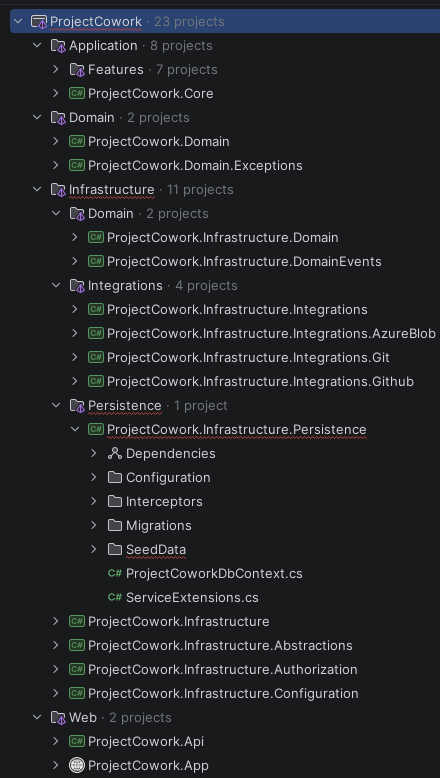
\includegraphics[scale=0.3]{rys04/org_proj.png}
    \caption{Struktura projektu}
    \label{fig:struktura_projekt}
\end{figure}

\section{Architektura systemu}
System został stworzony według specyfikacji architektury heksagonalnej z elementami DDD opisanymi w \cite{evans2015domain}, a także uzupełnionymi i przełożonymi na przykłady
praktyczne w \cite{vernon2016ddd}. Każda warstwa ma swoją jedną odpowiedzialność i nie jest zależna od warstwy od niej wyższej.
System został podzielony na aplikację serwerową i aplikację kliencką, które działają niezależnie od siebie. Warstwa serwerowa może zapewnić obsługę dla oprogramowania
innego niż tworzona aplikacja kliencka. 

\subsection{Diagram opisowy systemu}
System został podzielony na dwie aplikacje - serwerową i kliencką. Aplikacja serwerowa jest odpowiedzialna za logikę biznesową systemu, a aplikacja kliencka za interakcję z użytkownikiem.
Wizualizację opisową pokazano na rysunku \ref{fig:diag_opisowy}.
\begin{figure}[!htbp]
    \centering
    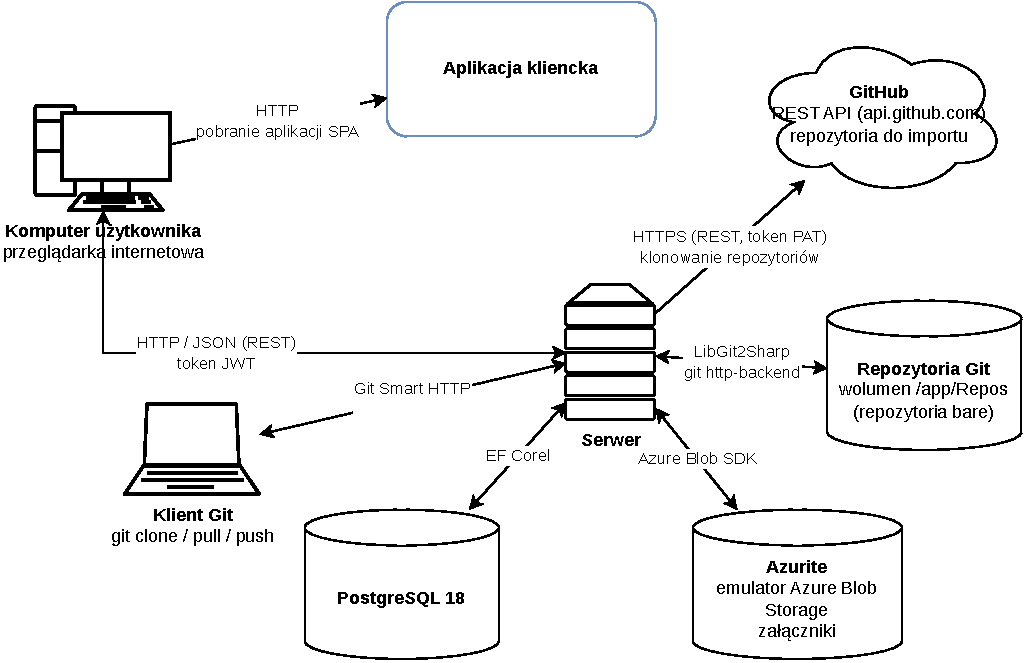
\includegraphics[scale=0.3]{rys04/diag_opis.pdf}
    \caption{Diagram opisowy systemu}
    \label{fig:diag_opisowy}
\end{figure}

\subsection{Diagram komponentów}
System został podzielony na kilka warstw, które dzielą się na podprojekty, które mają swoje pojedyncze odpowiedzialności. Warstwa domeny opisuje encje systemowe, enumy i wyjątki domenowe.
Warstwa infrastruktury zawiera integracje, wydarzenia domenowe, połączenie z bazą danych, konfigurację encji, uwierzytelnianie i pomniejsze klasy wspomagające.
Warstwa aplikacji zawiera logikę biznesową systemu, która jest wywoływana przez warstwę dostępową. Podzielona ona jest na moduły, gdzie każdy moduł odpowiada części domeny zawartej w warstwie domeny.
\begin{figure}[!htbp]
    \centering
    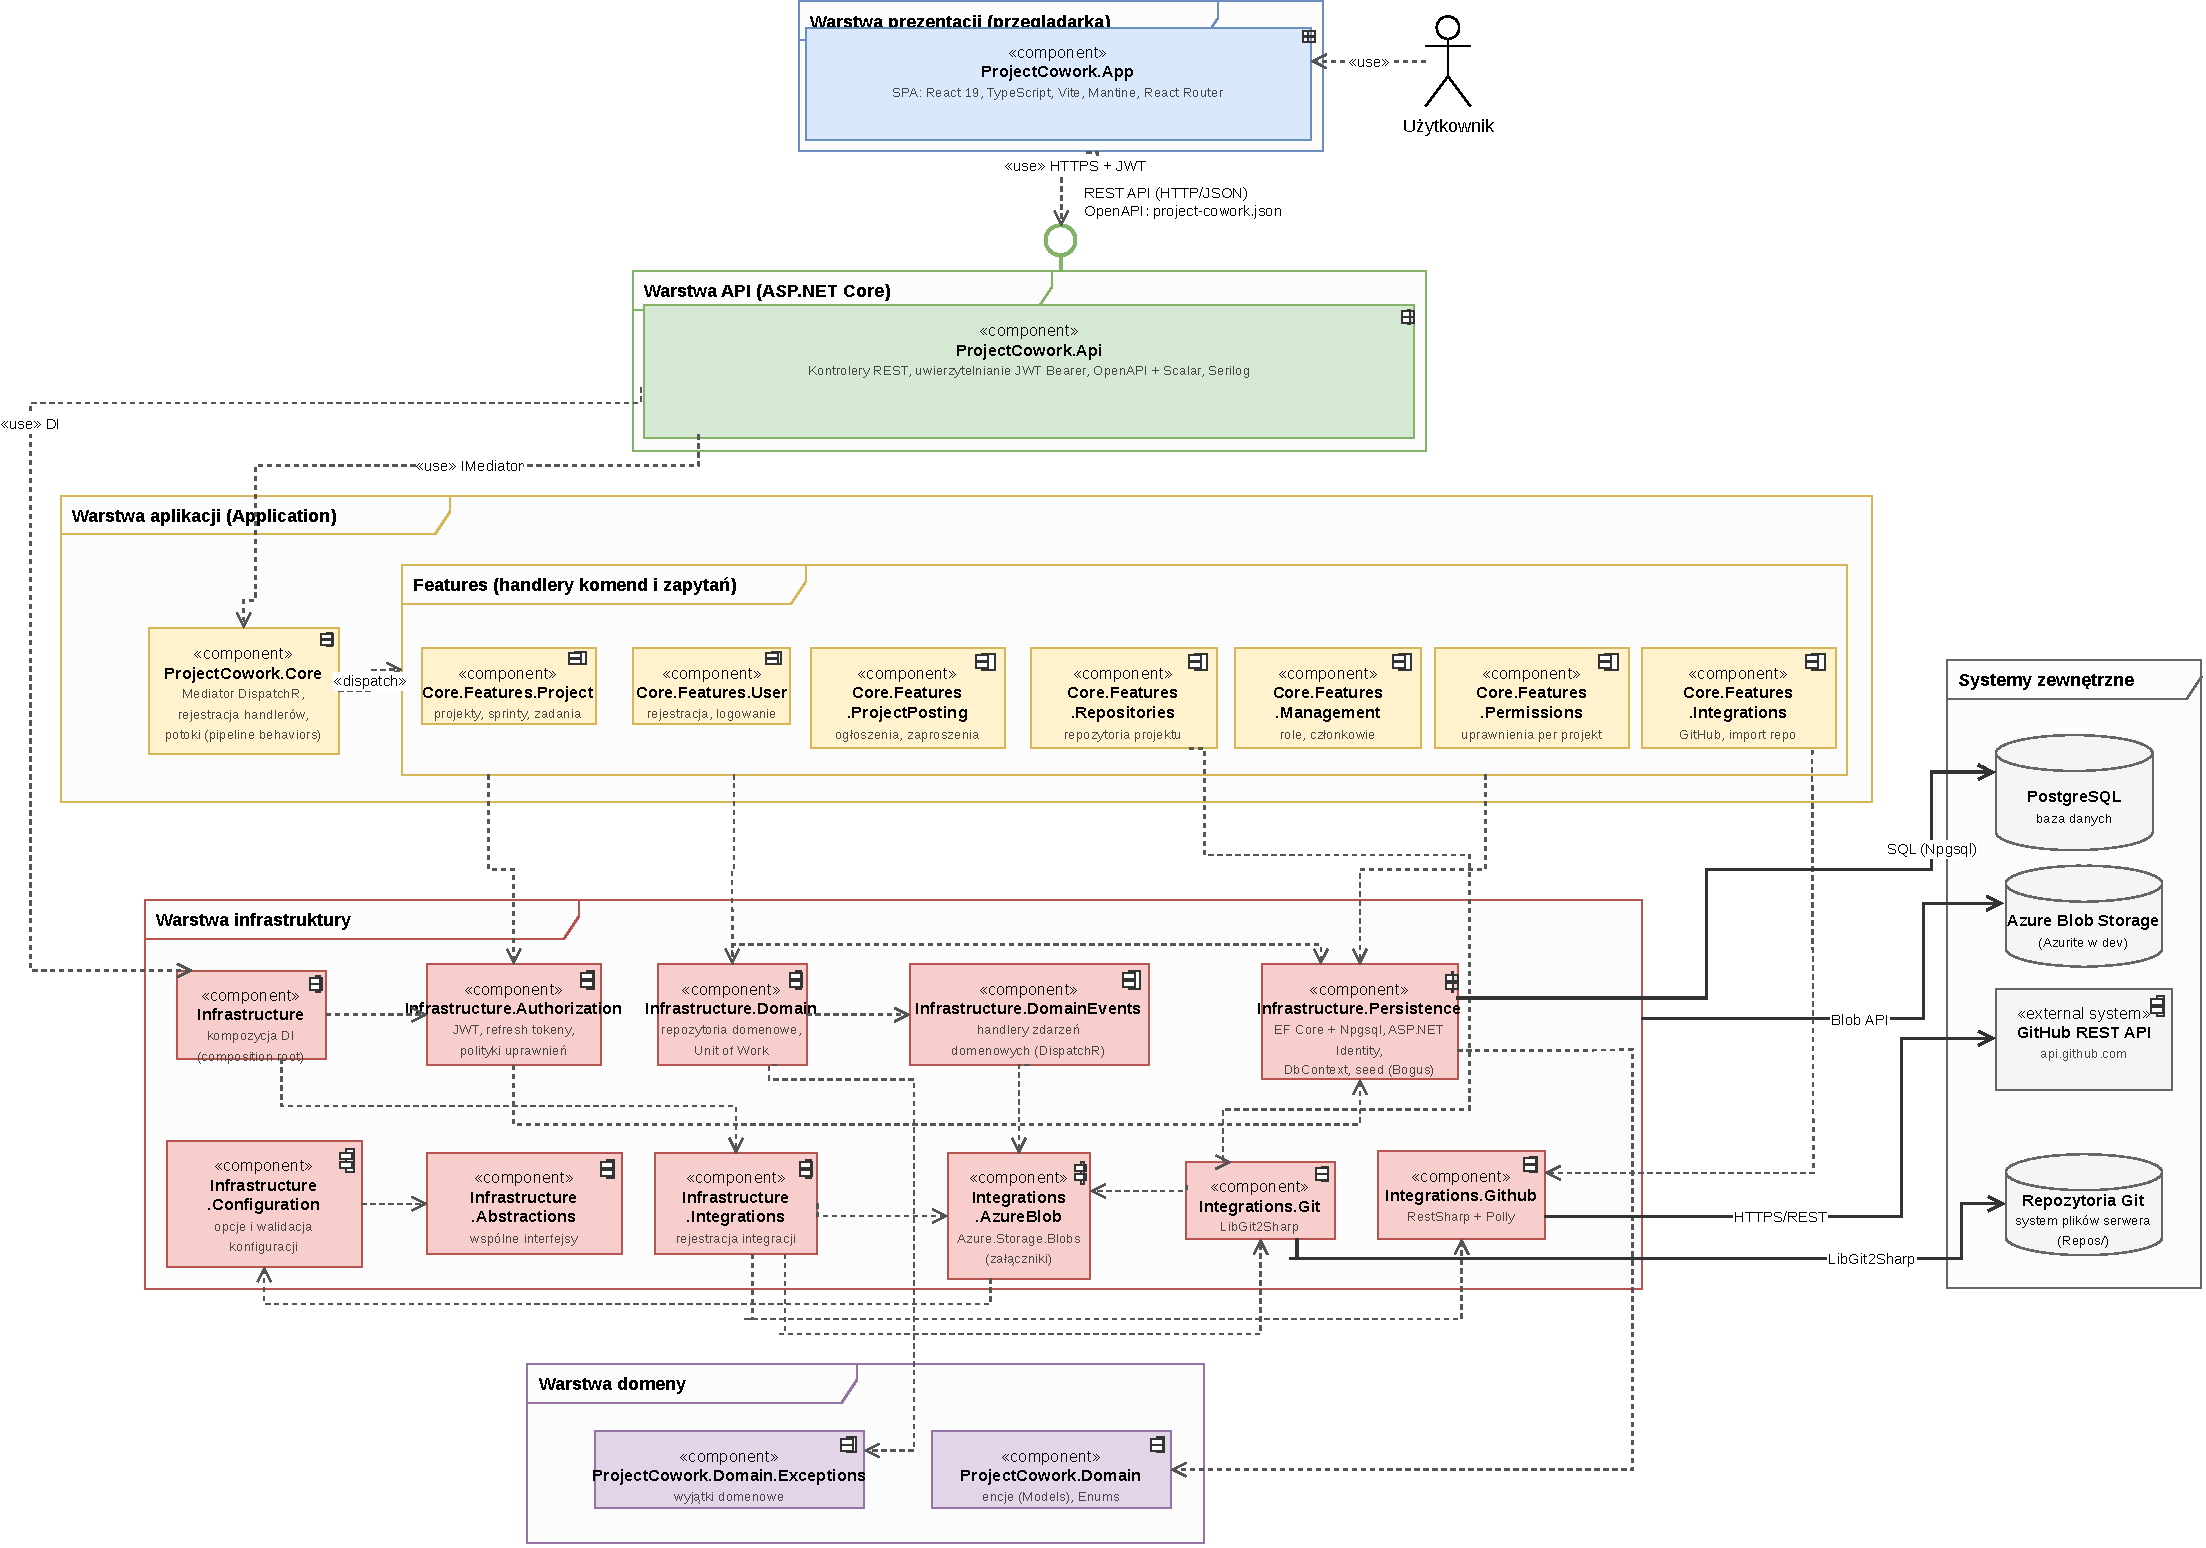
\includegraphics[scale=0.3]{rys04/diag_komp.pdf}
    \caption{Diagram komponentów systemu}
    \label{fig:diag_komp}
\end{figure}
\newpage
\subsection{Podejście projektowe}
W procesie projektowania aplikacji serwerowej zastosowano elementy podejścia \textit{DDD} (ang. \textit{Domain-Driven Design}) \cite{evans2015domain, vernon2016ddd}. Koncepcja ta zakłada ścisłe powiązanie struktury oprogramowania z docelową dziedziną biznesową poprzez wypracowanie tzw. języka wszechobecnego (ang. \textit{Ubiquitous Language}). Oznacza to, że terminologia stosowana bezpośrednio w kodzie źródłowym - w nazwach klas, metod oraz modułów -
jest tożsama z pojęciami używanymi przez ekspertów dziedzinowych oraz użytkowników końcowych. Takie podejście ułatwia zrozumienie działania systemu osobom nietechnicznym, upraszcza definiowanie nowych wymagań oraz zwiększa utrzymywalność projektu w miarę jego rozwoju.

Model domeny został rozdzielony na dwie części. Projekt \texttt{ProjectCowork.Domain} zawiera encje oraz typy wyliczeniowe, a projekt \texttt{ProjectCowork.Domain.Exceptions} wyjątki domenowe. Projekty te nie mają referencji do warstwy aplikacji, infrastruktury ani warstwy dostępowej, zależności w systemie są więc skierowane wyłącznie do domeny. Izolacja domeny od technologii nie jest jednak pełna. Encje \texttt{UserEntity} i \texttt{RoleEntity} dziedziczą po klasach \texttt{IdentityUser<Guid>} i \texttt{IdentityRole<Guid>} z biblioteki \texttt{ASP.NET Core Identity}, co pozwala wykorzystać gotowy mechanizm zarządzania kontami użytkowników bez tworzenia dodatkowej warstwy mapowania. Z kolei wyjątki domenowe przechowują kod statusu HTTP, który jest następnie zwracany przez warstwę dostępową. Są to świadome kompromisy, które upraszczają implementację kosztem czystości modelu.

Encje mają postać modelu anemicznego: są to klasy z publicznymi właściwościami i właściwościami nawigacyjnymi wykorzystywanymi przez \texttt{Entity Framework Core}, pozbawione logiki biznesowej. Logika ta została przeniesiona do klas agregatów w projekcie \texttt{ProjectCowork.Infrastructure.Domain}. Każdy agregat opakowuje encję główną, udostępnia statyczną metodę \texttt{Create} tworzącą poprawną encję oraz metody modyfikujące jej stan, które sprawdzają reguły biznesowe przed wprowadzeniem zmiany. Agregaty znajdują się w warstwie infrastruktury, ponieważ korzystają z mechanizmu publikowania zdarzeń opartego na bibliotece \texttt{DispatchR} oraz z rozszerzeń zapytań \texttt{Entity Framework Core}, które ładują wszystkie elementy agregatu z bazy danych.

W ramach projektowania w systemie wyróżniono następujące elementy wzorca DDD:
\begin{itemize}
    \item \textbf{Moduły funkcjonalne} - logika warstwy aplikacji została podzielona na moduły (\textit{Project}, \textit{Management}, \textit{Permissions}, \textit{ProjectPosting}, \textit{Repositories}, \textit{User}, \textit{Integrations}), z których każdy odpowiada za wyodrębniony fragment dziedziny. Podział ten nawiązuje do idei ograniczonych kontekstów (ang. \textit{Bounded Contexts}), jednak moduły korzystają ze wspólnego modelu domeny i jednego kontekstu bazy danych \texttt{ProjectCoworkDbContext}, nie są więc w pełni autonomiczne.
    \item \textbf{Encje (ang. \textit{Entities})} - obiekty posiadające unikalną tożsamość oraz własny cykl życia. W systemie tożsamość encji wyznacza identyfikator typu \texttt{Guid} (lub \texttt{int} w przypadku encji katalogu uprawnień). Encje, dla których istotna jest historia zmian, dziedziczą po klasie \texttt{BaseTrackedEntity}, której pola \texttt{CreatedAt} i \texttt{UpdatedAt} są uzupełniane automatycznie przez interceptor \texttt{Entity Framework Core} podczas zapisu.
    \item \textbf{Agregaty (ang. \textit{Aggregates})} - grupy powiązanych encji traktowane jako jedna jednostka spójności. Przykładem jest \texttt{ProjectAggregate}, który obejmuje projekt wraz z jego rolami i członkami oraz pilnuje niezmienników, takich jak istnienie dokładnie jednej roli domyślnej, unikalność nazw ról, zakaz usunięcia roli przypisanej do członków czy zakaz zmiany roli właściciela projektu. Analogicznie \texttt{SprintAggregate} sprawdza poprawność dat sprintu, a \texttt{TaskAggregate} nadaje zadaniom kolejne numery w obrębie projektu i ustawia datę ukończenia przy zmianie statusu. Ponieważ encje mają publiczne właściwości, wyłączność modyfikacji przez agregat nie jest wymuszana przez kompilator, lecz wynika z konwencji przyjętej w warstwie aplikacji.
    \item \textbf{Zdarzenia domenowe (ang. \textit{Domain Events})} - obiekty reprezentujące istotne fakty, które zaszły w systemie, np. \texttt{InvitationAcceptedEvent}, \texttt{SprintDeletedEvent}, \texttt{RepositoryDeletedEvent} czy \texttt{AttachmentAddedEvent}. Agregaty dziedziczące po klasie \texttt{AggregateRoot} rejestrują zdarzenia metodą \texttt{RaiseDomainEvent}, a handler komendy publikuje je przez mediator po wykonaniu operacji. Zdarzenia są obsługiwane w tym samym procesie i w ramach tego samego żądania. Nie zapewniają więc asynchroniczności, ale oddzielają operacje poboczne od głównej logiki. Przykładowo przyjęcie zaproszenia dodaje użytkownika do projektu w osobnym handlerze, a dodanie załącznika powoduje wysłanie pliku do usługi \texttt{Azure Blob Storage}.
\end{itemize}

W modelu nie zastosowano obiektów wartości (ang. \textit{Value Objects}). Proste atrybuty, takie jak daty, statusy czy priorytety zadań, są reprezentowane typami wbudowanymi (\texttt{DateOnly}, \texttt{DateTimeOffset}) oraz typami wyliczeniowymi, a ich walidacja odbywa się w agregatach.

Uzupełnieniem opisanych elementów w warstwie aplikacji jest zastosowanie wzorca \textit{CQRS} (ang. \textit{Command Query Responsibility Segregation}), który rozdziela operacje modyfikujące stan systemu (komendy) od operacji odczytujących dane (zapytania). Każdy moduł zawiera osobne katalogi \texttt{Commands} i \texttt{Queries}, a komendy i zapytania są obsługiwane przez osobne handlery. Rozdział ten ma charakter logiczny: obie strony korzystają z tej samej bazy danych i tego samego modelu, a zapytania nie przechodzą przez agregaty, tylko odczytują dane bezpośrednio z kontekstu bazy danych.

\section{Aplikacja serwerowa}
Aplikacja serwerowa, napisana w języku \texttt{C\#} opiera się na koncepcji architektury heksagonalnej z elementami DDD. Do komunikacji między warstwą dostępową API, a resztą warstw,
w celu lepszej enkapsulacji logiki, został użyty wzorzec \texttt{Mediator} \cite{mediator_pattern}. Wzorzec ten pozwala na komunikację między warstwami poprzez wysyłanie zapytań i komend, które są obsługiwane przez odpowiednie klasy handlerów.
Ogranicza to zależności między warstwami i nie korzystanie z interfejsów przy komunikacji między nimi. Wykorzystanie tego wzorca pozwoliło na 
zmiejszenie zależności między warstwami i wyczyściło metody w kontrolerach API, które teraz jedynie wykorzystują interfejs \texttt{IMediator} do wywoływania metod logiki biznesowej systemu.
Oprócz tego wzorca, system bardzo mocno wykorzystuje wbudowany we framework \texttt{.Net} mechanizm wstrzykiwania zależności, który pozwala na łatwe podmienianie implementacji interfejsów w systemie i ułatwia testowanie jednostkowe.
Instancje każdej klasy implementującej dany interfejs są tworzone w momencie uruchomienia aplikacji i wstrzykiwane do klas, które ich potrzebują. Każda z nich ma określony czas życia, co pozwala zoptymalizować wykorzystanie zasobów przy działaniu systemu.

\subsection{Diagram przepływu ze wzorcem Mediator-a}
Wzorzec \textit{Mediator} w wersji generycznej, opiera się na założeniu, że klasa żądająca danego zasobu lub chcąca zmodyfikować jakiś zasób, nie powinna znać implementacji klasy realizujacej takie żądanie.
Wzorzec ten pozwala na komunikację między warstwami poprzez wysyłanie zapytań i komend, które są obsługiwane przez odpowiednie klasy handlerów. Najczęstszym przypadkiem zastosowania tego wzorca jest implementacja wzorca \textit{CQRS}, który rozdziela logikę pobierania danych od logiki ich modyfikacji. W systemie zastosowano ten wzorzec, aby ograniczyć zależności między warstwami i nie korzystać z interfejsów przy komunikacji między nimi.
Na rysunku \ref{fig:diag_mediator} przedstawiono diagram przepływu danych w systemie z wykorzystaniem wzorca \textit{Mediator} w celu lepszego zobrazowania działania tego wzorca. Jako przykład przyjęto proces inicjalizacji nowego, pustego repozytorium w projekcie.

\begin{figure}[!htbp]
    \centering
    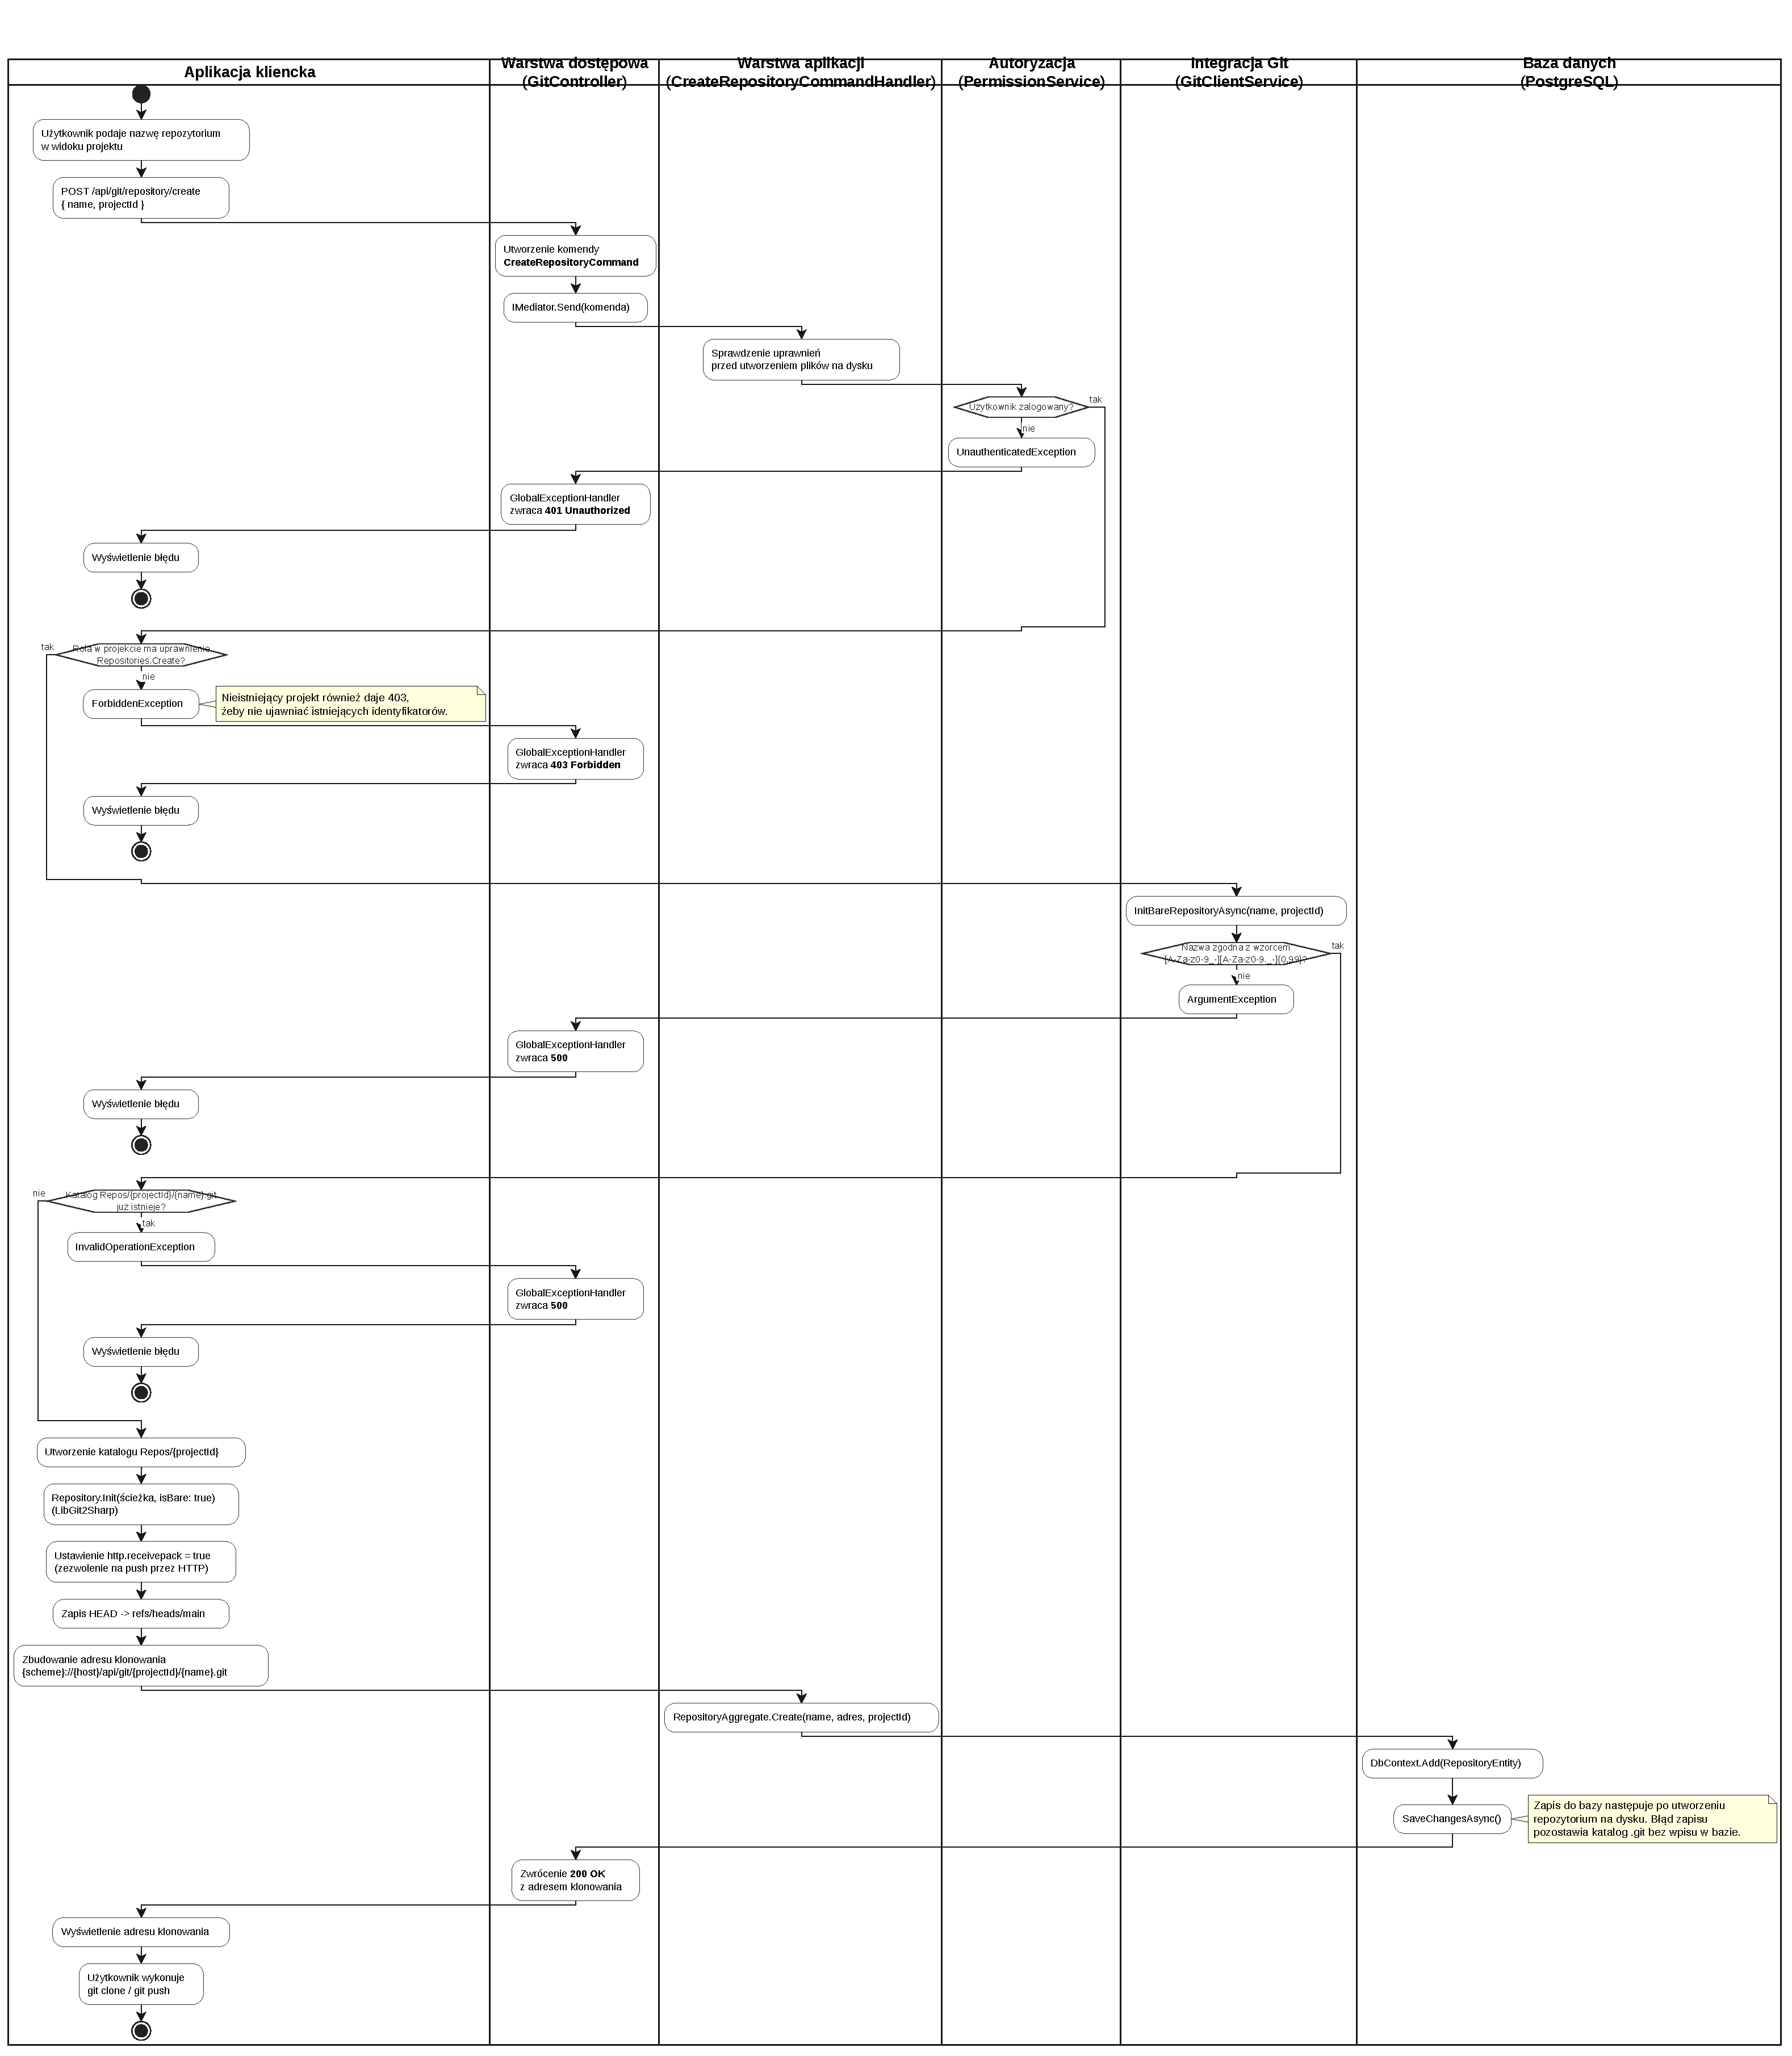
\includegraphics[scale=0.3]{rys04/diag_przeplyw.pdf}
    \caption{Diagram przepływu danych w systemie z wykorzystaniem wzorca Mediator}
    \label{fig:diag_mediator}
\end{figure}

\subsection{Warstwa domenowa}
Warstwa domenowa odpowiada tylko i wyłącznie za model domeny systemu, który w tym przypadku jest anemiczny i dopiero jest wzbogacany w warstwie infrastruktury. Każda encja posiada swoje własności
i definiuje relacje z innymi encjami. W tej warstwie również znajdują się wyjątki domenowe, które są wykorzystywane w logice biznesowej.

\subsection{Warstwa infrastruktury}
W warstwie infrastruktury znajdują się wszystkie integracje z systemami zewnętrznymi, konfiguracja encji w bazie danych, konfiguracja \textit{ORM},
konfiguracja uwierzytelniania i autoryzacji, konfiguracja zdarzeń domenowych i pomniejsze klasy wspomagające działanie systemu takie jak chociażby Agregaty wykorzystywane w logice biznesowej.
Warstwa ta, jak wskazuje nazwa, jest odpowiedzialna za cześć typowo infrastrukturalną systemu i jest niezależna od logiki biznesowej.

\subsection{Warstwa aplikacji}
Warstwa aplikacji została zgodnie z założeniami \textit{CQRS} \cite{CQRS}. Zamiast zwykłych serwisów (klas zawierających metody logiki biznesowej), zgodnie z tym 
wzorcem logika pobierania danych i ich zapisu została od siebie rozdzielona. Każdy moduł systemu posiada katalog \texttt{Commands}, w którym znajdują się klasy komend, które są wywoływane w momencie kiedy użytkownik chce zmienić stan systemu.
Każda komenda posiada swój handler, który jest wywoływany przez wzorzec \texttt{Mediator} i w nim znajduje się logika biznesowa, która zmienia stan systemu. Analogicznie, każdy moduł posiada katalog \texttt{Queries}, w którym znajdują się klasy zapytań, które są wywoływane w momencie kiedy użytkownik chce pobrać dane z systemu.


\subsection{Warstwa dostępowa}
Warstwa dostępowa została stworzona jako API w architekturze \textit{REST} \cite{rest_redhat}. Aplikacja składa się z kilku klas kontrolerów, 
które wywołują odpowiednie metody logiki biznesowej poprzez wzorzec \texttt{Mediator}. Każdy kontroler odpowiada za jeden moduł systemu i posiada metody, które odpowiadają na żądania HTTP,
zwracając odpowiedni kod statusu HTTP i dane w formacie \textit{JSON}, lub sam kod statusu. W warstwie tej został również skonfigurowany Globalna klasa obsługująca wyjątki, która
przechwytuje wszystkie wyjątki z systemu i zwraca odpowiedni kod statusu HTTP w zalezności od wyjątku. 

\section{Aplikacja kliencka}
Aplikacja kliencka, znajdująca się w folderze \textit{Web/ProjectCowork.App} została napisana we frameworku \texttt{React.js} za pomocą języka \texttt{Typescript}.
Architektura aplikacji została podzielona na tzw. \texttt{Hooks}, gdzie zdefiniowane są połączenia z Api, 
\texttt{Features}, gdzie zdefiniowane są strony dla każdego modułu aplikacji, \texttt{Auth}, gdzie znajduje się obsługa sesji zalogowanego użytkownika
i reszta gdzie znajdują się funkcje pomocnicze, takie jak obsługa głównego
stylu strony i tego jak się zachowuje strona w momencie kiedy użytkownik jest zalogowany lub nie.

%TODO: Dodac ss samego projektu frontu

\section{Konteneryzacja}
System został skonteneryzowany za pomocą narzędzia \texttt{Docker} \cite{docker_docs}. Każda z aplikacji, serwerowa i kliencka, posiada swój własny plik konfiguracyjny \texttt{Dockerfile}, który określa jak ma zostać zbudowany obraz kontenera.
To wszystko jest zintegrowane poprzez konfigurację w pliku \textit{compose.yaml}, co sprawia, że żeby uruchomić system, wystarczy wykonać jedną komendę \texttt{docker compose up --build} w katalogu \textit{src}.
Plik konfiguracyjny przedstawiono na listingu \ref{lst:compose}.

\begin{lstlisting}[basicstyle=\footnotesize\ttfamily, captionpos=t, caption={Plik \texttt{compose.yaml} uruchamiający system}, label={lst:compose}]
services:
  postgres:
    image: postgres:18-alpine
    restart: unless-stopped
    environment:
      POSTGRES_DB: ${POSTGRES_DB:-ProjectCowork}
      POSTGRES_USER: ${POSTGRES_USER:-postgres}
      POSTGRES_PASSWORD: ${POSTGRES_PASSWORD:-postgres}
    ports:
      - "5432:5432"
    volumes:
      # Od PostgreSQL 18 dane trzymane są w /var/lib/postgresql/<wersja>/docker.
      - postgres-data:/var/lib/postgresql
    healthcheck:
      test: ["CMD-SHELL", "pg_isready -U $${POSTGRES_USER} -d $${POSTGRES_DB}"]
      interval: 5s
      timeout: 5s
      retries: 10

  azurite:
    image: mcr.microsoft.com/azure-storage/azurite:latest
    restart: unless-stopped
    command: azurite-blob --blobHost 0.0.0.0 --blobPort 10000 --loose --skipApiVersionCheck
    ports:
      - "10000:10000"
    volumes:
      - azurite-data:/data

  projectcowork.api:
    image: projectcowork.api
    build:
      context: .
      dockerfile: Web/ProjectCowork.Api/Dockerfile
    restart: unless-stopped
    depends_on:
      postgres:
        condition: service_healthy
      azurite:
        condition: service_started
    environment:
      ASPNETCORE_ENVIRONMENT: ${ASPNETCORE_ENVIRONMENT:-Development}
      ASPNETCORE_HTTP_PORTS: "8080"
      ConnectionStrings__DefaultConnection: "Host=postgres;Port=5432;Database=${POSTGRES_DB:-ProjectCowork};Username=${POSTGRES_USER:-postgres};Password=${POSTGRES_PASSWORD:-postgres}"
      Integrations__BlobStorage__ConnectionString: "DefaultEndpointsProtocol=http;AccountName=devstoreaccount1;AccountKey=Eby8vdM02xNOcqFlqUwJPLlmEtlCDXJ1OUzFeyLM+SR4UcR+JdBqDBwqD4l4hxsRJtCeZ6EPgnYQ==;BlobEndpoint=http://azurite:10000/devstoreaccount1;"
      Cors__AllowedOrigins__0: "http://localhost:${APP_PORT:-3000}"
      # Kontenery działają po HTTP, więc ciasteczko z refresh tokenem nie może mieć flagi Secure.
      # Front i API na localhost z różnymi portami to ta sama "strona", więc wystarcza SameSite=Lax.
      AuthCookie__SameSite: Lax
      AuthCookie__Secure: "false"
    ports:
      - "${API_PORT:-8080}:8080"
    volumes:
      # Repozytoria git tworzone przez aplikację (Repos/{projectId}/{nazwa}.git).
      - git-repos:/app/Repos

  projectcowork.app:
    image: projectcowork.app
    build:
      context: .
      dockerfile: Web/ProjectCowork.App/Dockerfile
      args:
        VITE_API_URL: "http://localhost:${API_PORT:-8080}"
    restart: unless-stopped
    depends_on:
      - projectcowork.api
    ports:
      - "${APP_PORT:-3000}:80"

volumes:
  postgres-data:
  azurite-data:
  git-repos:
\end{lstlisting}
Ze względu na specyfikę działania systemu, w pliku konfigurowana jest baza danych \texttt{PostgreSQL}, która jest wykorzystywana przez aplikację serwerową, a także kontener z usługą \texttt{Azurite}, która emuluje działanie usługi \texttt{Azure Blob Storage} w środowisku lokalnym.
Dodatkowo, przez to że system współdziała z systemem kontroli wersji \textit{Git}, w kontenerze konfigurowany jest również ten system.